\documentclass[aspectratio=169]{beamer}
	\usepackage[utf8]{inputenc}		% required for umlauts
	\usepackage[english]{babel}		% language
	%\usepackage[sfdefault]{roboto}	% enable sans serif font roboto
	%\usepackage{libertine}			% enable this on Windows to allow for microtype
	\usepackage[T1]{fontenc}		% required for output of umlauts in PDF

	\usepackage{mathtools}		% required for formulas

	\usepackage{caption}		% Customize caption aesthetics
	\usepackage{tcolorbox}		% fancy colored boxes
	\usepackage{xcolor}			% Highlighting
	\usepackage{soul}
	\usepackage{graphicx}		% required to insert images
	\usepackage[space]{grffile} % insert images baring a filename which contains spaces
	\usepackage{float}			% allow to forcefully set the location of an object

	\usepackage[tracking=true]{microtype} % required to change character spacing

	\usepackage[style=numeric,backend=biber]{biblatex}
	\usepackage{hyperref}		% insert clickable references

	\usepackage{datetime}		% flexible date specification
	\newcommand{\leadingzero}[1]{\ifnum#1<10 0\the#1\else\the#1\fi}
	\newcommand{\todayddmmyyyy}{\leadingzero{\day}.\leadingzero{\month}.\the\year}
	\newcommand{\mathcolorbox}[2]{\colorbox{#1}{$\displaystyle #2$}}

	\usepackage{geometry}
	\usepackage{scrextend}		% allow arbitrary indentation

	\usepackage{color}

	\addbibresource{../literature.bib}

	\setbeamercolor{title}{fg=orange}
	\setbeamertemplate{title}{
		\color{orange}
		\textbf{\inserttitle}
	}
	\setbeamercolor{tableofcontents}{fg=orange}
	\setbeamercolor{section in toc}{fg=black}
	\setbeamercolor{subsection in toc}{fg=black}
	\setbeamertemplate{frametitle}{
		%\vspace{0.5em}
		\color{orange}
		\begin{center}
			\textbf{\insertframetitle} \\
			{\small \insertframesubtitle}
		\end{center}
	}
	\setbeamertemplate{footline}[text line]{
  		\parbox{\linewidth}{
			  \color{gray}
			  \vspace*{-1em}
			  PSRC 2018
			  \hfill
			  Gordian (\href{mailto:gordian.edenhofer@gmail.com}{gordian.edenhofer@gmail.com})
			  \hfill
			  \insertpagenumber
		}
	}
	\setbeamertemplate{navigation symbols}{}
	\setbeamertemplate{itemize item}{\color{black}$\bullet$}
	\setbeamertemplate{itemize subitem}{\color{black}$\circ$}
	\setbeamercolor{block title}{fg=black}
	\captionsetup{font=scriptsize,labelfont={bf,scriptsize}}

	\titlegraphic{
		\vspace{-8.5em}
		\hspace{20em}
		
\includegraphics[width=\textwidth,height=.2\textheight,keepaspectratio]{{{../res/Excellence Cluster Universe logo}}}
	}
	\title{Optimization of Particle Identification}
	\subtitle{The Analysis Software behind Particle Discoveries}
	\author[Edenhofer]{\href{mailto:gordian.edenhofer@gmail.com}{Gordian Edenhofer}}
	\institute[LMU]{
		Working Group of Prof.~Dr.~Kuhr \\
		Faculty of Physics \\
		Excellence Cluster Universe
	}
	\date[PSRC 2018]{Physics Student Research Conference, 09. June 2018}
	\subject{Particle Physics}


\begin{document}

\begin{frame}[plain]
	\titlepage
\end{frame}
\note{
	\begin{itemize}
		\item Superior particle identification
		\item Better event topology analysis
		\item Improved particle physics validation at Belle \uppercase\expandafter{\romannumeral 2}
	\end{itemize}

	\begin{itemize}
		\item Event topology (particle abundances, kinematics)
		\item Utilize interdependence of detector variables
	\end{itemize}
}

\section[Belle \uppercase\expandafter{\romannumeral 2}]{Belle \uppercase\expandafter{\romannumeral 2} Experiment}
\begin{frame}
	\frametitle{\insertsection}

	\begin{columns}[T]
		\begin{column}{.6\textwidth}
			\vspace{3em}
			\begin{itemize}
				\item Standard Model validation
				\item Electron-, positron-accelerator
				\item $B$-Meson factory
			\end{itemize}
			\begin{itemize}
				\item Asymmetric beams at $\sqrt{S} = 10.58 \mathrm{~GeV}$
				\item Integrated luminosity of $50 \mathrm{~ab}^{-1}$
				\item $4.4 \cdot 10^{10}$ events
				%\item Instantaneous luminosity of $8 \cdot 10^{35} \mathrm{cm}^{-2} \mathrm{s}^{-1}$
				%\item Cross section: $~10 \mathrm{\mu m} \times 60 \mathrm{nm}$
			\end{itemize}
		\end{column}
		\begin{column}{.4\textwidth}
			\begin{figure}
				\centering
				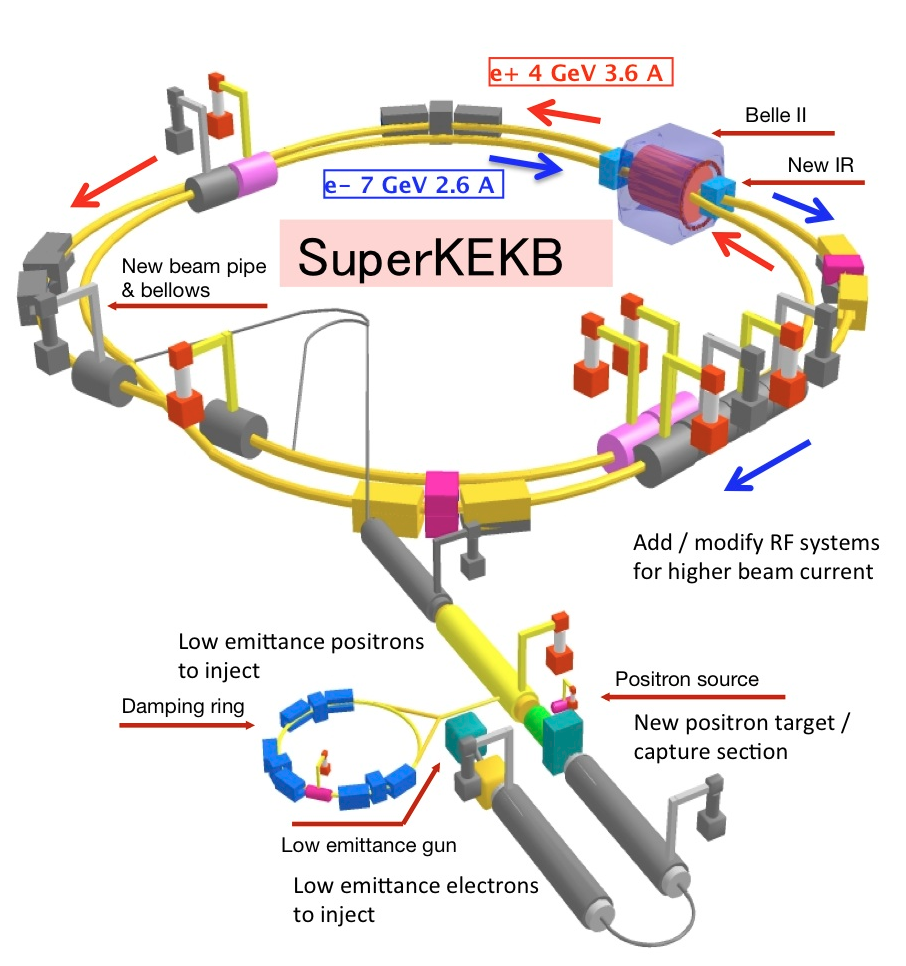
\includegraphics[width=\textwidth,height=0.6\textheight,keepaspectratio]{{{../res/Belle 2 accelerator: SuperKEKB}}}
				\caption{Sketch of the Belle \uppercase\expandafter{\romannumeral 2} accelerator SuperKEKB. Adapted from \cite{Belle2Collaboration:SuperKEKBSketch}.}
			\end{figure}
		\end{column}
	\end{columns}
\end{frame}

\subsection{Detector Systems}
\begin{frame}
	\frametitle{\insertsection}
	\framesubtitle{\insertsubsection}

	\begin{columns}[T]
		\begin{column}{.54\textwidth}
			\begin{figure}
				\centering
				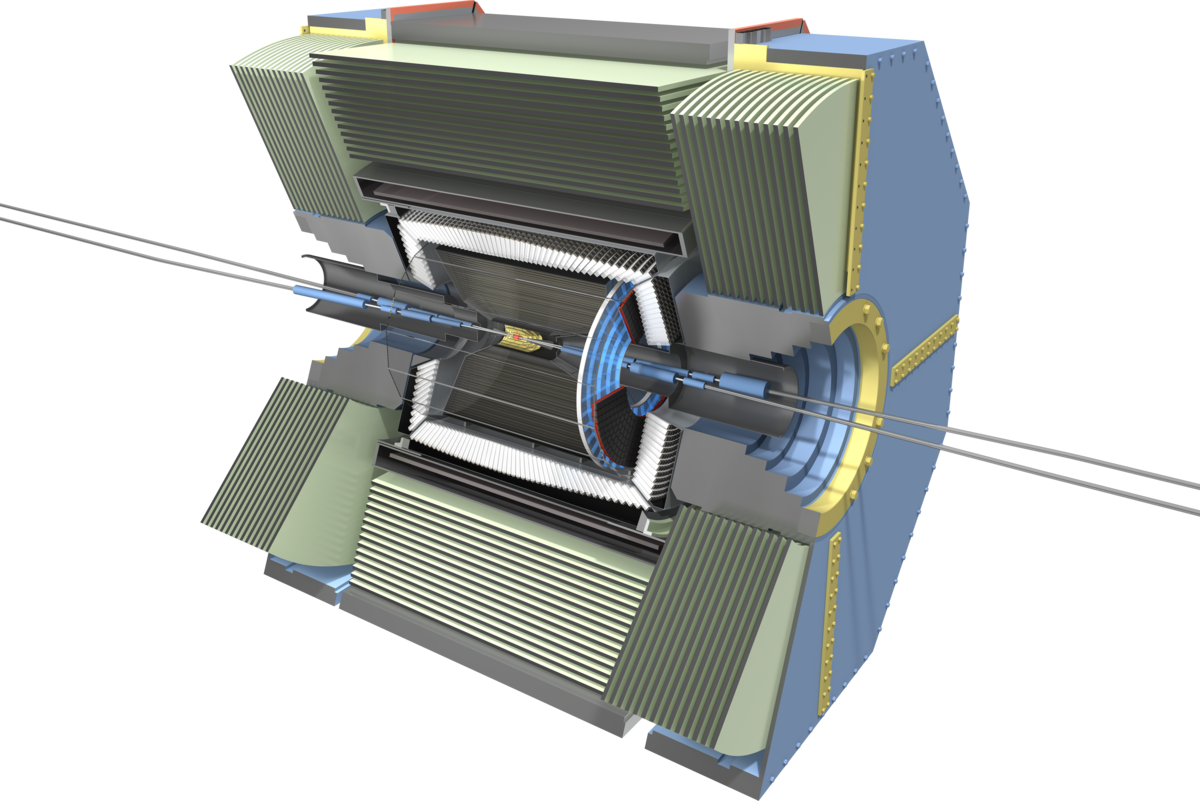
\includegraphics[width=\textwidth,height=0.5\textheight,keepaspectratio]{{{../res/Belle 2 detector}}}
				\caption{Belle \uppercase\expandafter{\romannumeral 2} detector. Taken from \cite{Belle2Collaboration:Belle2as3DSketch}.}
			\end{figure}
		\end{column}
		\begin{column}{.45\textwidth}
			\vspace{1.5em}
			\begin{itemize}
				\item \textbf{P}i\textbf{X}el \textbf{D}etector
				\item \textbf{S}ilicon \textbf{V}ertex \textbf{D}etector
				\item \textbf{C}entral \textbf{D}rift \textbf{C}hamber
				\item \textbf{T}ime \textbf{O}f \textbf{P}ropagation counter
				\item \textbf{A}erogel \textbf{RICH} counter
				\item \textbf{E}lectromagnetic \textbf{C}a\textbf{L}orimeter
				\item $\boldsymbol{K}^0_{\boldsymbol{L}}$/$\boldsymbol{\mu}$ detector
			\end{itemize}
		\end{column}
	\end{columns}
\end{frame}

\section[Statistics]{Identification}
\subsection{Bayes}
\begin{frame}
	\frametitle{\insertsection}
	\framesubtitle{\insertsubsection}

	\begin{alertblock}{Bayes' Theorem}
		\centering
		$\mathcolorbox{yellow}{P(A|B) = \frac{P(B|A) \cdot P(A)}{P(B)}}$
	\end{alertblock}
	\vspace{1em}

	The likelihood of a particle may vary depending on its
	\begin{itemize}
		\item abundance
		\item angle between particle and beam
		\item transverse momentum
		\item point of detection
		\item \ldots
	\end{itemize}
\end{frame}

\section{Identification}
\subsection{Inventory}
\begin{frame}
	\frametitle{\insertsection}
	\framesubtitle{\insertsubsection}

	\begin{columns}[T]
		\begin{column}{.49\textwidth}
			\begin{figure}
				\centering
				\includegraphics[width=\textwidth,height=0.55\textheight,keepaspectratio]{{{../res/sample/General Purpose Statistics: True Particle Abundances in the K+-Data}}}
				\caption{True particle abundance in a simulated $D$-decay.}
			\end{figure}
		\end{column}
		\begin{column}{.49\textwidth}
			\begin{figure}
				\centering
				\includegraphics[width=\textwidth,height=0.55\textheight,keepaspectratio]{{{../res/sample/Multivariate Bayesian Approach: Multi-axes Histogram of pt, cosTheta}}}
				\caption{Multi-axis histogram depending on $p_t$ and $cos(\Theta)$ in a simulated $D$-decay.}
			\end{figure}
		\end{column}
	\end{columns}
\end{frame}

\subsection{Idea}
\begin{frame}
	\frametitle{\insertsection}
	\framesubtitle{\insertsubsection}

	\begin{columns}[T]
		\begin{column}{.49\textwidth}
			\textbf{Current approach:} \\
			\begin{itemize}
				\item Take ratio of particle likelihood over pion likelihood, e.g. $electronID = \mathcal{L}_{e} / (\mathcal{L}_{e} +\mathcolorbox{yellow}{\mathcal{L}_{\pi}})$
				\item Perform selection on ID, e.g. $electronID > 0.2$
			\end{itemize}
		\end{column}
		\begin{column}{.49\textwidth}
			\textbf{Investigated alternative:} \\
			\begin{itemize}
				\item Multivariate dependencies, e.g. $electronID(p_t, \Theta) = \frac{\mathcal{L}_{e} \cdot C_{e}(p_t, \Theta)}{\sum \limits_{x \in {K, e, \dots}} \mathcal{L}_{x} \cdot  C_{x}(p_t, \Theta)}$
				\item Adaptable priors $C_{x}(a, b)$ incorporating the abundance and further detector variables like $p_t$ and $\Theta$
			\end{itemize}
		\end{column}
	\end{columns}
\end{frame}

\subsection{ROC \& PPV}
\begin{frame}
	\frametitle{\insertsection}
	\framesubtitle{\insertsubsection}

	\begin{figure}
		\centering
		\includegraphics[width=\textwidth,height=0.65\textheight,keepaspectratio]{{{../res/charged 01/Diff Statistics: K Identification via PID, by pt & cos(Theta)}}}
		\caption{Kaon Identification via PID and Bayes by $p_t$ \& $\cos(\Theta)$ for a generic decay.}
	\end{figure}
\end{frame}

\subsection{Confusion Matrix}
\begin{frame}
	\frametitle{\insertsection}
	\framesubtitle{\insertsubsection}

	\begin{figure}
		\centering
		\includegraphics[width=\textwidth,height=0.6\textheight,keepaspectratio]{{{../res/charged 01/Diff Heatmap: Heatmap of epsilonPID Matrix for an exclusive Cut via PID, by pt & cos(Theta)}}}
		\caption{Heatmaps of row-wised normed confusion matrices for PID and Bayes by $p_t$ \& $\cos(\Theta)$, showing the particle identification and confusion rates for a generic decay.}
	\end{figure}
\end{frame}

{
	\setbeamertemplate{footline}[text line]{
  		\parbox{\linewidth}{
			  \color{black}
			  \vspace*{-5em}
			  PSRC 2018
			  \hfill
			  Gordian (\href{mailto:gordian.edenhofer@gmail.com}{gordian.edenhofer@gmail.com})
			  \hfill
			  \color{gray}
			  \insertpagenumber
		}
	}

	\subsection{Conclusion}
	\begin{frame}
		\frametitle{\insertsection}
		\framesubtitle{\insertsubsection}

		\begin{itemize}
			\item Same detector data but utilizing knowledge about decay
			\item Incorporate multiple detector variables
			\item Flexible a priori probabilities
		\end{itemize}
		$\Rightarrow$ Improved particle identification with less false positives
	\end{frame}
}

\section*{Bibliography}
\begin{frame}
	\frametitle{\insertsection}

	\printbibliography
\end{frame}

\section{Appendix}
\subsection{Terminology}
\begin{frame}
	\frametitle{\insertsection}
	\framesubtitle{\insertsubsection}

	\begin{columns}
		\begin{column}{0.47\textwidth}
			\begin{block}{\textbf{T}rue \textbf{P}ositive \textbf{R}ate (TPR)}
				Elements which are correctly identified as being correct
			\end{block}
			\begin{block}{\textbf{T}rue \textbf{N}egative \textbf{R}ate (TNR)}
				Elements which are correctly identified as being incorrect
			\end{block}
		\end{column}
		\begin{column}{0.5\textwidth}
			\begin{block}{\textbf{F}alse \textbf{P}ositive \textbf{R}ate (FPR)}
				Elements which are incorrectly identified as being correct
			\end{block}
			\begin{block}{\textbf{F}alse \textbf{N}egative \textbf{R}ate (FNR)}
				Elements which are incorrectly identified as being incorrect
			\end{block}
		\end{column}
	\end{columns}
	\vspace{2em}
	\mathcolorbox{yellow}{
		\begin{tabular}{l|ll}
			Veracity & True = correct & False = incorrect \\
			Identification & Positive = accepted & Negative = rejected
		\end{tabular}
	}
\end{frame}

\subsection{Existing Methods}
\begin{frame}
	\frametitle{\insertsection}
	\framesubtitle{\insertsubsection}

	\begin{columns}
		\begin{column}{0.47\textwidth}
			\begin{table}
				\begin{tabular}{l|l}
					pionID & $\mathcal{L}_{\pi} / (\mathcolorbox{yellow}{\mathcal{L}_{\pi}} + \mathcal{L}_{K})$ \\
					kaonID & $\mathcal{L}_{K} / (\mathcal{L}_{K} +\mathcolorbox{yellow}{\mathcal{L}_{\pi}})$ \\
					protonID & $\mathcal{L}_{p} / (\mathcal{L}_{p} +\mathcolorbox{yellow}{\mathcal{L}_{\pi}})$ \\
					electronID & $\mathcal{L}_{e} / (\mathcal{L}_{e} +\mathcolorbox{yellow}{\mathcal{L}_{\pi}})$ \\
					muonID & $\mathcal{L}_{\mu} / (\mathcal{L}_{\mu} +\mathcolorbox{yellow}{\mathcal{L}_{\pi}})$ \\
					deuteronID & $\mathcal{L}_{d} / (\mathcal{L}_{d} +\mathcolorbox{yellow}{\mathcal{L}_{\pi}})$
				\end{tabular}
				\caption{ParticleID detector variables for selection and further analysis.}
			\end{table}
		\end{column}
		\begin{column}{0.5\textwidth}
			\begin{table}
				\begin{tabular}{l|l}
					pidProbabilityPion & $\mathcal{L}_{\pi} / \mathcal{L}_{all}$ \\
					pidProbabilityKaon & $\mathcal{L}_{K} / \mathcal{L}_{all}$ \\
					pidProbabilityProton & $\mathcal{L}_{p} / \mathcal{L}_{all}$ \\
					pidProbabilityElectron & $\mathcal{L}_{e} / \mathcal{L}_{all}$ \\
					pidProbabilityMuon & $\mathcal{L}_{\mu} / \mathcal{L}_{all}$ \\
					pidProbabilityDeuteron & $\mathcal{L}_{d} / \mathcal{L}_{all}$ \\
					\hline
					\multicolumn{2}{c}{$\mathcal{L}_{all} = \sum \limits_{x \in {\pi, K, p, e, \mu, d}} \mathcal{L}_{x}$}
				\end{tabular}
				\caption{Likelihood-Ratios for particle selection and further analysis.}
			\end{table}
		\end{column}
	\end{columns}
\end{frame}

\end{document}
